\documentclass{article}

\usepackage[margin=1in]{geometry}

% \documentclass{article}

\usepackage{graphicx} % Required for inserting images
\usepackage{amsmath}
\usepackage{amsfonts}
\usepackage{amsthm}
% \usepackage{amssymb}
\usepackage{mathtools}
\usepackage{xcolor}
\usepackage{hyperref}
\usepackage{tikz}
\usepackage{pgfplots}
\usepackage{booktabs}
\usepackage{algorithm}%
\usepackage{algorithmicx}%
\usepackage{algpseudocode}%
\usepackage{listings}%
\usepackage{url}
\usepackage[most]{tcolorbox}
\newtcbox{\mymath}[1][]{%
	nobeforeafter, math upper, tcbox raise base,
	enhanced, colframe=blue!30!black,
	colback=blue!30, boxrule=1pt,
	#1}

% \usepackage[sort]{natbib}
\frenchspacing

%%%%%%%%%%%---SETME-----%%%%%%%%%%%%%
%replace @@ with the submission number submission site.
\newcommand{\thiswork}{INF$^2$\xspace}
%%%%%%%%%%%%%%%%%%%%%%%%%%%%%%%%%%%%


%\newcommand{\rev}[1]{{\color{olivegreen}#1}}
\newcommand{\rev}[1]{{#1}}


\newcommand{\JL}[1]{{\color{cyan}[\textbf{\sc JLee}: \textit{#1}]}}
\newcommand{\JW}[1]{{\color{orange}[\textbf{\sc JJung}: \textit{#1}]}}
\newcommand{\JY}[1]{{\color{blue(ncs)}[\textbf{\sc JSong}: \textit{#1}]}}
\newcommand{\HS}[1]{{\color{magenta}[\textbf{\sc HJang}: \textit{#1}]}}
\newcommand{\CS}[1]{{\color{navy}[\textbf{\sc CShin}: \textit{#1}]}}
\newcommand{\SN}[1]{{\color{olive}[\textbf{\sc SNoh}: \textit{#1}]}}

%\def\final{}   % uncomment this for the submission version
\ifdefined\final
\renewcommand{\JL}[1]{}
\renewcommand{\JW}[1]{}
\renewcommand{\JY}[1]{}
\renewcommand{\HS}[1]{}
\renewcommand{\CS}[1]{}
\renewcommand{\SN}[1]{}
\fi

%%% Notion for baseline approaches %%% 
\newcommand{\baseline}{offloading-based batched inference\xspace}
\newcommand{\Baseline}{Offloading-based batched inference\xspace}


\newcommand{\ans}{attention-near storage\xspace}
\newcommand{\Ans}{Attention-near storage\xspace}
\newcommand{\ANS}{Attention-Near Storage\xspace}

\newcommand{\wb}{delayed KV cache writeback\xspace}
\newcommand{\Wb}{Delayed KV cache writeback\xspace}
\newcommand{\WB}{Delayed KV Cache Writeback\xspace}

\newcommand{\xcache}{X-cache\xspace}
\newcommand{\XCACHE}{X-Cache\xspace}


%%% Notions for our methods %%%
\newcommand{\schemea}{\textbf{Expanding supported maximum sequence length with optimized performance}\xspace}
\newcommand{\Schemea}{\textbf{Expanding supported maximum sequence length with optimized performance}\xspace}

\newcommand{\schemeb}{\textbf{Optimizing the storage device performance}\xspace}
\newcommand{\Schemeb}{\textbf{Optimizing the storage device performance}\xspace}

\newcommand{\schemec}{\textbf{Orthogonally supporting Compression Techniques}\xspace}
\newcommand{\Schemec}{\textbf{Orthogonally supporting Compression Techniques}\xspace}



% Circular numbers
\usepackage{tikz}
\newcommand*\circled[1]{\tikz[baseline=(char.base)]{
            \node[shape=circle,draw,inner sep=0.4pt] (char) {#1};}}

\newcommand*\bcircled[1]{\tikz[baseline=(char.base)]{
            \node[shape=circle,draw,inner sep=0.4pt, fill=black, text=white] (char) {#1};}}


\begin{document}

\title{Countering Election Sway: \\ Strategic Algorithms in Friedkin-Johnsen Dynamics}
%\author{Charalampos E. Tsourakakis\\ ctsourak@bu.edu \\ Boston University}

\author{Dragos Ristache \\ dragosr@bu.edu \\ Boston University \and Fabian Spaeh \\ fspaeh@bu.edu \\ Boston University \and  Charalampos E. Tsourakakis \\ ctsourak@bu.edu \\ Boston University}

\maketitle

\begin{abstract}
    \begin{abstract}  
Test time scaling is currently one of the most active research areas that shows promise after training time scaling has reached its limits.
Deep-thinking (DT) models are a class of recurrent models that can perform easy-to-hard generalization by assigning more compute to harder test samples.
However, due to their inability to determine the complexity of a test sample, DT models have to use a large amount of computation for both easy and hard test samples.
Excessive test time computation is wasteful and can cause the ``overthinking'' problem where more test time computation leads to worse results.
In this paper, we introduce a test time training method for determining the optimal amount of computation needed for each sample during test time.
We also propose Conv-LiGRU, a novel recurrent architecture for efficient and robust visual reasoning. 
Extensive experiments demonstrate that Conv-LiGRU is more stable than DT, effectively mitigates the ``overthinking'' phenomenon, and achieves superior accuracy.
\end{abstract}  
\end{abstract}

\section{Introduction}
\label{sec:intro}
\section{Introduction}


\begin{figure}[t]
\centering
\includegraphics[width=0.6\columnwidth]{figures/evaluation_desiderata_V5.pdf}
\vspace{-0.5cm}
\caption{\systemName is a platform for conducting realistic evaluations of code LLMs, collecting human preferences of coding models with real users, real tasks, and in realistic environments, aimed at addressing the limitations of existing evaluations.
}
\label{fig:motivation}
\end{figure}

\begin{figure*}[t]
\centering
\includegraphics[width=\textwidth]{figures/system_design_v2.png}
\caption{We introduce \systemName, a VSCode extension to collect human preferences of code directly in a developer's IDE. \systemName enables developers to use code completions from various models. The system comprises a) the interface in the user's IDE which presents paired completions to users (left), b) a sampling strategy that picks model pairs to reduce latency (right, top), and c) a prompting scheme that allows diverse LLMs to perform code completions with high fidelity.
Users can select between the top completion (green box) using \texttt{tab} or the bottom completion (blue box) using \texttt{shift+tab}.}
\label{fig:overview}
\end{figure*}

As model capabilities improve, large language models (LLMs) are increasingly integrated into user environments and workflows.
For example, software developers code with AI in integrated developer environments (IDEs)~\citep{peng2023impact}, doctors rely on notes generated through ambient listening~\citep{oberst2024science}, and lawyers consider case evidence identified by electronic discovery systems~\citep{yang2024beyond}.
Increasing deployment of models in productivity tools demands evaluation that more closely reflects real-world circumstances~\citep{hutchinson2022evaluation, saxon2024benchmarks, kapoor2024ai}.
While newer benchmarks and live platforms incorporate human feedback to capture real-world usage, they almost exclusively focus on evaluating LLMs in chat conversations~\citep{zheng2023judging,dubois2023alpacafarm,chiang2024chatbot, kirk2024the}.
Model evaluation must move beyond chat-based interactions and into specialized user environments.



 

In this work, we focus on evaluating LLM-based coding assistants. 
Despite the popularity of these tools---millions of developers use Github Copilot~\citep{Copilot}---existing
evaluations of the coding capabilities of new models exhibit multiple limitations (Figure~\ref{fig:motivation}, bottom).
Traditional ML benchmarks evaluate LLM capabilities by measuring how well a model can complete static, interview-style coding tasks~\citep{chen2021evaluating,austin2021program,jain2024livecodebench, white2024livebench} and lack \emph{real users}. 
User studies recruit real users to evaluate the effectiveness of LLMs as coding assistants, but are often limited to simple programming tasks as opposed to \emph{real tasks}~\citep{vaithilingam2022expectation,ross2023programmer, mozannar2024realhumaneval}.
Recent efforts to collect human feedback such as Chatbot Arena~\citep{chiang2024chatbot} are still removed from a \emph{realistic environment}, resulting in users and data that deviate from typical software development processes.
We introduce \systemName to address these limitations (Figure~\ref{fig:motivation}, top), and we describe our three main contributions below.


\textbf{We deploy \systemName in-the-wild to collect human preferences on code.} 
\systemName is a Visual Studio Code extension, collecting preferences directly in a developer's IDE within their actual workflow (Figure~\ref{fig:overview}).
\systemName provides developers with code completions, akin to the type of support provided by Github Copilot~\citep{Copilot}. 
Over the past 3 months, \systemName has served over~\completions suggestions from 10 state-of-the-art LLMs, 
gathering \sampleCount~votes from \userCount~users.
To collect user preferences,
\systemName presents a novel interface that shows users paired code completions from two different LLMs, which are determined based on a sampling strategy that aims to 
mitigate latency while preserving coverage across model comparisons.
Additionally, we devise a prompting scheme that allows a diverse set of models to perform code completions with high fidelity.
See Section~\ref{sec:system} and Section~\ref{sec:deployment} for details about system design and deployment respectively.



\textbf{We construct a leaderboard of user preferences and find notable differences from existing static benchmarks and human preference leaderboards.}
In general, we observe that smaller models seem to overperform in static benchmarks compared to our leaderboard, while performance among larger models is mixed (Section~\ref{sec:leaderboard_calculation}).
We attribute these differences to the fact that \systemName is exposed to users and tasks that differ drastically from code evaluations in the past. 
Our data spans 103 programming languages and 24 natural languages as well as a variety of real-world applications and code structures, while static benchmarks tend to focus on a specific programming and natural language and task (e.g. coding competition problems).
Additionally, while all of \systemName interactions contain code contexts and the majority involve infilling tasks, a much smaller fraction of Chatbot Arena's coding tasks contain code context, with infilling tasks appearing even more rarely. 
We analyze our data in depth in Section~\ref{subsec:comparison}.



\textbf{We derive new insights into user preferences of code by analyzing \systemName's diverse and distinct data distribution.}
We compare user preferences across different stratifications of input data (e.g., common versus rare languages) and observe which affect observed preferences most (Section~\ref{sec:analysis}).
For example, while user preferences stay relatively consistent across various programming languages, they differ drastically between different task categories (e.g. frontend/backend versus algorithm design).
We also observe variations in user preference due to different features related to code structure 
(e.g., context length and completion patterns).
We open-source \systemName and release a curated subset of code contexts.
Altogether, our results highlight the necessity of model evaluation in realistic and domain-specific settings.






 \section{Related work} 
\label{sec:rel}
\putsec{related}{Related Work}

\noindent \textbf{Efficient Radiance Field Rendering.}
%
The introduction of Neural Radiance Fields (NeRF)~\cite{mil:sri20} has
generated significant interest in efficient 3D scene representation and
rendering for radiance fields.
%
Over the past years, there has been a large amount of research aimed at
accelerating NeRFs through algorithmic or software
optimizations~\cite{mul:eva22,fri:yu22,che:fun23,sun:sun22}, and the
development of hardware
accelerators~\cite{lee:cho23,li:li23,son:wen23,mub:kan23,fen:liu24}.
%
The state-of-the-art method, 3D Gaussian splatting~\cite{ker:kop23}, has
further fueled interest in accelerating radiance field
rendering~\cite{rad:ste24,lee:lee24,nie:stu24,lee:rho24,ham:mel24} as it
employs rasterization primitives that can be rendered much faster than NeRFs.
%
However, previous research focused on software graphics rendering on
programmable cores or building dedicated hardware accelerators. In contrast,
\name{} investigates the potential of efficient radiance field rendering while
utilizing fixed-function units in graphics hardware.
%
To our knowledge, this is the first work that assesses the performance
implications of rendering Gaussian-based radiance fields on the hardware
graphics pipeline with software and hardware optimizations.

%%%%%%%%%%%%%%%%%%%%%%%%%%%%%%%%%%%%%%%%%%%%%%%%%%%%%%%%%%%%%%%%%%%%%%%%%%
\myparagraph{Enhancing Graphics Rendering Hardware.}
%
The performance advantage of executing graphics rendering on either
programmable shader cores or fixed-function units varies depending on the
rendering methods and hardware designs.
%
Previous studies have explored the performance implication of graphics hardware
design by developing simulation infrastructures for graphics
workloads~\cite{bar:gon06,gub:aam19,tin:sax23,arn:par13}.
%
Additionally, several studies have aimed to improve the performance of
special-purpose hardware such as ray tracing units in graphics
hardware~\cite{cho:now23,liu:cha21} and proposed hardware accelerators for
graphics applications~\cite{lu:hua17,ram:gri09}.
%
In contrast to these works, which primarily evaluate traditional graphics
workloads, our work focuses on improving the performance of volume rendering
workloads, such as Gaussian splatting, which require blending a huge number of
fragments per pixel.

%%%%%%%%%%%%%%%%%%%%%%%%%%%%%%%%%%%%%%%%%%%%%%%%%%%%%%%%%%%%%%%%%%%%%%%%%%
%
In the context of multi-sample anti-aliasing, prior work proposed reducing the
amount of redundant shading by merging fragments from adjacent triangles in a
mesh at the quad granularity~\cite{fat:bou10}.
%
While both our work and quad-fragment merging (QFM)~\cite{fat:bou10} aim to
reduce operations by merging quads, our proposed technique differs from QFM in
many aspects.
%
Our method aims to blend \emph{overlapping primitives} along the depth
direction and applies to quads from any primitive. In contrast, QFM merges quad
fragments from small (e.g., pixel-sized) triangles that \emph{share} an edge
(i.e., \emph{connected}, \emph{non-overlapping} triangles).
%
As such, QFM is not applicable to the scenes consisting of a number of
unconnected transparent triangles, such as those in 3D Gaussian splatting.
%
In addition, our method computes the \emph{exact} color for each pixel by
offloading blending operations from ROPs to shader units, whereas QFM
\emph{approximates} pixel colors by using the color from one triangle when
multiple triangles are merged into a single quad.



\section{Proposed methods} 
\label{sec:proposed}
% \paragraph{Problem Formulation.} 

Our work focuses on the {\it median} of the equilibrium
opinion vector (or simply, the median opinion),
which we defined in Equation~\eqref{eq:fj2}.
The median opinion indicates exactly where
the majority lies, and therefore directly
relates to winning or loosing an election.
In this section, we introduce different
strategies that can be used to optimize
the median in a specific direction.
%
For simplicity, we only
formally provide an objective with the goal to
maximize the median, but the minimization
objective can be defined analogously.
%
We introduce the following optimization problem
where we want to maximize the increase in the
median opinion under a fixed budget $k$ of the resistance parameter change. 
For any agent $u \in V$, we may change
its resistance $\alpha_u$, but not its
innate opinion $s_u$; this reflects a simple
attack on someone's susceptibility to persuasion
\cite{abebe2020opinion}.
%
We measure distances between the original
resistance vector $\alpha$ and modified
resistances $\alpha'$ in an arbitrary
$\ell_p$ norm $\| \cdot \|_p$, and we obtain
one optimization problem for each value
of $p \ge 0$.

\begin{tcolorbox}
\begin{problem}[\textsc{Maximizing the Median under FJ Dynamics}]
\label{prob:max-median} Let $(\alpha, W, s)$ be a network
of generalized FJ dynamics and $k$ be a budget on the change of resistance values. Maximize the objective
$\mathrm{Median}(x^\star(\alpha', W, s))$
where $\alpha' \in [0,1]^n$ is a vector of resistances
such that $\|\alpha' - \alpha\|_p \le k$

%where $\| \cdot \|_p$ denotes the $\ell_p$ norm.
\end{problem}
\end{tcolorbox}


We also consider the dual of this problem, which
addresses the question of how many stooges are
needed in order to flip the median beyond
a certain threshold $\theta$. This problem directly addresses the question of what budget is necessary in order to win an election. 

\begin{tcolorbox}
\begin{problem}[\textsc{Flipping the Median under FJ Dynamics}]
\label{prob:elections}
Let $(\alpha, W, s)$ be a network of generalized FJ dynamics
and $\theta \in \R$ a threshold.
Minimize $\|\alpha' - \alpha\|_p$ such that
$\alpha' \in [0,1]^n$ is a vector of resistances
with $\mathrm{Median}(x^\star(\alpha, W, s)) > \theta$.
\end{problem}
\end{tcolorbox}


The two norms of interest in this work are for $p\in\{0,1\}$. The $\ell_0$
pseudo-norm is defined as
$\| \alpha - \alpha' \|_0 = |\{ u \in V : \alpha_u \not= \alpha'_u \}|$
which counts the number of distinct elements.
This corresponds to targeting
$k$ nodes and converting them into stooges. The variant with $p=1$ has also received attention in the literature~\cite{chan2021hardness}. 


\begin{figure}
    \centering
    \small
    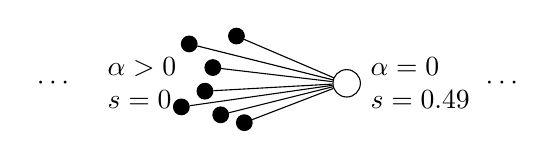
\begin{tikzpicture}
        \node at (-1.7, -0.5) {$\cdots$};
        \node at (4, -0.5) {$\cdots$};
        \node[align=left] at (-0.6, -0.5) {$\alpha>0$\\ $s=0$};
        \node[inner sep=2pt, draw=black, circle, fill] (u1) at (0, 0) {};
        \node[inner sep=2pt, draw=black, circle, fill] (u2) at (0.6, 0.1) {};
        \node[inner sep=2pt, draw=black, circle, fill] (u3) at (-0.1, -0.8) {};
        \node[inner sep=2pt, draw=black, circle, fill] (u4) at (0.3, -0.3) {};
        \node[inner sep=2pt, draw=black, circle, fill] (u5) at (0.2, -0.6) {};
        \node[inner sep=2pt, draw=black, circle, fill] (u6) at (0.4, -0.9) {};
        \node[inner sep=2pt, draw=black, circle, fill] (u7) at (0.7, -1) {};
        \node[inner sep=3.5pt, draw=black, circle, label={[align=left]right:$\alpha=0$\\ $s=0.49$}] (v) at (2, -0.5) {};
        \draw (u1) to (v);
        \draw (u2) to (v);
        \draw (u3) to (v);
        \draw (u4) to (v);
        \draw (u5) to (v);
        \draw (u6) to (v);
        \draw (u7) to (v);
    \end{tikzpicture}
    \caption{An example showcasing challenges in
    Problems~\ref{prob:max-median}
    and \ref{prob:elections}. We show
    an isolated component in a larger
    graph, where the black vertices
    on the left have innate innate opinion
    $0$, but are only connected to the
    white vertex on the right with innate
    opinion $0.5$ but resistance $0$.}
    \label{fig:example}
\end{figure}

We can trivially convert an algorithm for
Problem~\ref{prob:max-median} into an
algorithm addressing Problem~\ref{prob:elections}
by a binary search over the budgets.
%
A natural heuristic for these optimization
problems is the greedy algorithm, which
in each iteration designates a new node
as a stooge, and the selection is made 
such that it maximizes the increase in the
median opinion.
%
This solves both problems at the same time,
as we can keep adding stooges until we
flip the median opinion across the
threshold $\theta$.
%
However, Figure~\ref{fig:example} exemplifies
a difficulty with this approach:
Initially, it may seem that using the
the white node on the right as a stooge
and changing its resistance to $\alpha=1$
results in a big increase in the
median opinions. However,
if the objective is to move the
median beyond a threshold of $\theta=0.5$,
this modification is in vain, since it
does not move any opinion past the
threshold. Furthermore, employing
more stooges in the shown isolated
component does not help with our objective either.
%
Greedily selecting stooges is therefore
problematic. Other problems with
the greedy algorithm are its inefficiency
on large graphs, since we need to identify
the best node to become a stooge in
each iteration. We will later
discuss the greedy algorithm and how to
apply it on large networks.
We show formally that our targeted
problems are hard to approximate in
Theorem~\ref{thm:hardness}.
In the remainder of this section,
we analyze the hardness and discuss different heuristics
to address Problems~\ref{prob:max-median}
and Problem~\ref{prob:elections}.

\subsection{Hardness of Problem~\ref{prob:max-median}}

Our first key result is that Problem~\ref{prob:max-median} is computationally hard. Specifically, we establish the following inapproximability result. 

\begin{theorem}
    \label{thm:hardness}
    Problem~\ref{prob:max-median}
    for $p=0$
    is inapproximable
    to any multiplicative factor
    unless $\mathsf{P} = \mathsf{NP}$.
\end{theorem}


The proof is based on a novel reduction from the set cover problem~\cite{williamson2011design}, which we defer to the appendix. Furthermore, a straight-forward corollary of our reduction shows that this result carries over not only to the $\frac{1}{2}$-percentile which is the median, but to any $q$-quantile for $0 < q < 1$.

\begin{corollary}
\label{cor:quantile}
Let $(\alpha, W, s)$ be a network of generalized FJ  dynamics,
let $k$ be a budget and $0 < q < 1$  be any fixed quantile value.
The problem of maximizing the $q$-th quantile of $x^\star(\alpha', W, s)$ subject to $\|\alpha' - \alpha\|_0 \le k$ (akin to Problem~\ref{prob:max-median} for $q=\frac{1}{2}$) cannot be approximated to any multiplicative factor unless $\mathsf{P} = \mathsf{NP}$.
\end{corollary}

On the other hand,
for the special case of directed trees,
we can solve this problem optimally
in polynomial time using dynamic programming,
which we show in the appendix.


\subsection{Huber M-Estimator}



To circumvent the hardness of
maximizing the median
and avoid the aforementioned
issues with the greedy algorithm,
we want to turn our attention on
a continuous approximation of the median which
makes our objectives amenable to iterative methods.
The median as a function represents a piecewise-defined
function characterized by inherent discontinuities.
This non-differentiable nature precludes the applicability
of gradient-based optimization techniques, which
fundamentally rely on smooth and continuous objectives
to ensure convergence towards a (potentially locally)
optimal solution. 
Continuous approaches do not commit
to stooges, which could lead to problems as the one
shown in Figure~\ref{fig:example}.
Our approach for tackling Problem~\ref{prob:elections} is
formally stated in Algorithm~\ref{alg:huber-gd}.
However, before delving into details, we
want to motivate our continuous relaxation. We start by
using the Huber M-estimator to derive smooth,
differentiable formulations for the median,
akin to how the softmax function serves as a smooth
approximation for the maximum value
\cite{brown2001smoothed,hampel2011smoothing}.
The Huber M-estimator is a robust statistical estimator that
combines properties of both the sample mean and the sample
median to produce an estimate that is resistant to outliers.
The key idea is to minimize a function of residuals that is
quadratic for small residuals but linear for large residuals.
The Huber loss is parameterized by a tuning constant $c$ and is defined as 
\[
    H_c(x) =
    \begin{cases} 
        \frac 1 2 x^2 & \textrm{if } |x| \le c \\
        c \cdot \left(|x| - \frac 1 2 c\right) & \textrm{otherwise} .
    \end{cases} 
\]
%
The tuning constant $c$ determines the point at which the loss switches from being quadratic to linear. The intuition behind Huber's M-estimator being a good proxy for the median lies in its loss function, which is less sensitive to outliers than the mean. The mean averages all values equally, giving high influence to outliers, while the median is resistant to outliers but does not take into account ``how far'' the other points are from it.  To find Huber's M-estimator $\hat y$ for a data set \( \{ x_1, x_2, \ldots, x_n \} \), we
solve the minimization
\begin{align}
    \label{eq:y-star}
    \hat y = \hat y_c = \min_y \sum_{i=1}^{n} H_c(x_i - y) .
\end{align}
The extreme values of $c$
give us either the median or
the mean, as $\hat y_0 = \mathrm{Median}(\bx)$
and $\hat y_\infty = \mathrm{Mean}(\bx)$. After introducing the robust and continuous
approximation to the median, we now state a continuous adaption of
Problem~\ref{prob:elections} with $\ell_1$ budget constraint~\cite{chan2021hardness}


%
\begin{formulation}[\textsc{Minimal Budget for Election Influence via FJ Dynamics}]
\label{prob:elections_formal} 
Consider a network of FJ dynamics represented by $(\alpha, W, s)$, where $c \ge 0$ is the Huber loss parameter, and $\theta \in \R$ represents a threshold.  Minimize $\|\alpha' - \alpha\|_1$, subject to the condition that $\alpha' \in [0, 1]^n$ is a vector of resistances, and $\hat y(\alpha') \ge \theta$, where $\hat y(\alpha')$ is defined as $\min_y \sum_{i=1}^n H_c(x^\star_i(\alpha', W, s) - y)$.



% Given an FJ opinion dynamic and ,
% how many nodes do we have to make stooges
% such that $\min_y \sum_i H_c(x_i - y) > \frac 1 2$, where
% $\bx$ are the equilibrium opinions?
% \fabian{we need to use $\|\alpha' - \alpha\|_1$
% as budget for the continuous approaches. How about:
% Let $(\alpha, W, s)$ be a network of FJ dynamics, and
% $\theta \in \R$ a threshold. Minimize
% $\|\alpha' - \alpha\|_1$ such that
% $\alpha' \in [0, 1]^n$ is a vector of resistances
% with $\hat y(\alpha') \ge \theta$
% where $\hat y(\alpha') = \min_y \sum_{i=1}^n H_c(x^\star_i(\alpha', W, s) - y)$.}
\end{formulation}

\iffalse
\spara{Greedy does not work well using Huber's loss.} \labis{visualization will help here? O/w define left, right}
We could try an algorithm that greedily
chooses stooges in order to maximize $H_c(\bx)$.
However, such an algorithm may perform
poorly, at least in theory.
Imagine a large opinion dynamic, where
a $K_{k, n, 1}$ is an isolated tripartite
graph with $n \gg k \gg 1$. The left vertices have resistance
$1$, the middle vertices resistance $\approx 0$,
and the right vertex resistance $1$.
The innate opinions are $0$ for all vertices.
Now, choosing the right vertex 
changes the equilibrium opinions to
$\frac 1 2$ for the $n$ nodes in the middle.
This gives us a potentially big increase in
the mean, and potentially in the median
depending on the rest of the graph.
However, we will never be able to push
a substantial number of the $n$ middle
vertices beyond an opinion of $\frac 1 2$.
Thus, this increase was meaningless
and we should not have picked the right vertex,
but some other vertex in the remainder
of the graph.
\fabian{I think this could also serve
as an example why Problems 2 and 3 are
hard. We could move this ahead and
just state here that we also get an increase
in the mean, so the approx. objective
with huber's loss cannot overcome this
issue. Also, what purpose do the $k$
vertices on the left serve?}
\fi

\paragraph{Gradient Formulation}
We now show how to derive a gradient
for the Huber's M-estimator $\hat y$.
Since the M-Estimator itself is the
result of optimization problem in
Equation~\ref{eq:y-star},
we first need to analyze properties
of the minimizer.
To this end,
we define the set
$I = \{i : |x^\star_i - \hat y| < c\}$.
For any $y \in \mathbb R$,
\[
    \sum_{i} H_c(x^\star_{i} - y) =
    c \sum_{i \notin I} \left(|x^\star_i - y| - \frac 1 2 c\right)
    + \frac 1 2 \sum_{i \in I} (x^\star_i - y)^2
\]
and we thus have the identity
\begin{multline*}
    0 = \frac{\partial}{\partial \hat y} \sum_i H_c(x^\star_i - \hat y)
    = -c \sum_{i \notin I} \mathrm{sgn}(x^\star_i - \hat y)
    - \sum_{i \in I} (x^\star_i - \hat y) \\
    \iff
    \hat y = \frac 1 {|I|} \Big(
      c \sum_{i \notin I} \mathrm{sgn}(x^\star_i - \hat y) +
      \sum_{i \in I} x^\star_i \Big) .
\end{multline*}
Assuming $x^\star_i \not= \hat y$ for all $i$, we thus obtain
\[
    \frac{\partial \hat y}{\partial x^\star_i} =
    \frac 1 {|I|} 1_{[i \in I]}
\]
where we denote with $1_{[\mathrm{cond}(u)]} \in \R^n$
the vector which is $1$ in the rows corresponding
to $u$ where $\mathrm{cond}(u)$ is true and $0$, otherwise.
%
It remains to compute the derivative          \def\transMatrix{W}
$ \partial \bx^\star / \partial \alpha $
where $\bx^\star = (I - (I - A) \transMatrix)^+ A \bs$ are the equilibrium opinions and
$A = \mathrm{Diag}(\alpha)$.
Let
\begin{align*}
    X =
    I - (I - A) \transMatrix
    \quad\textrm{and}\quad
    \bx^\star =
    X^+ A \bs .
\end{align*}
Note that we can obtain $\bx^\star$ without
computing the full pseudoinverse $X^+$
by solving the least-squares problem
$\min_\bx \| X \bx - A \bs \|_2$.
We want to show that
\[
    \frac{\partial \bx^\star}{\partial \alpha} =
    X^+ \mathrm{Diag}(\bs) - X^+ \mathrm{Diag}(\transMatrix \bx^\star) .
\]
By the product rule,
\[
    \frac{\partial \bx^\star}{\partial \alpha} =
    \frac{\partial X^+ A \bs}{\partial \alpha} =
    X^+ \otimes \frac{A \bs}{\partial \alpha} +
    \frac{\partial X^+}{\partial \alpha} \otimes A \bs .
\]
We evaluate both terms. The first term is easy:
\[
    X^+ \otimes \frac{\partial A \bs}{\partial \alpha} =
    X^+ \otimes \mathrm{Diag}(\bs) =
    X^+ \mathrm{Diag}(\bs) .
\]
For the second term, we apply the chain rule:
\[
    \frac{\partial X^+}{\partial \alpha} =
    \frac{\partial X^+}{\partial X} \otimes
    \frac{\partial X}{\partial \alpha} =
    \frac{\partial X^+}{\partial X} \otimes
    \frac{\partial A \transMatrix}{\partial \alpha} .
\]
We  use that
$\partial X^+_{ij} / \partial L_{ab} = -X^+_{ia} X^+_{bj}$
since $X$ has full rank.
Furthermore, 
\[
    \frac{\partial (AM)_{ab}}{\partial a_k}
    = 1_{[a = k]} M_{ab} .
\]
Thus,
\begin{align*}
    \left( \frac{\partial X^+}{\partial X} \otimes
    \frac{\partial A \transMatrix}{\partial \alpha} \right)_{ijk}
    &= - \sum_{a,b} X^+_{ia} X^+_{bj} 1_{[a = k]} M_{ab} \\
    &= - \sum_{b} X^+_{ik} X^+_{bj} M_{kb}
    = - X^+_{ik} (\transMatrix X^+)_{kj}
\end{align*}
and
\begin{align*}
    \left( \frac{\partial X^+}{\partial \alpha} \otimes A \bs \right)_{ik} &=
    - \sum_j X^+_{ik} (\transMatrix X^+)_{kj} (A \bs)_j \\ &=
    - X^+_{ik} (\transMatrix X^+ A \bs)_{k} =
    - X^+_{ik} (\transMatrix x^\star)_{k}
\end{align*}
which means
$\partial X^+ / \partial \alpha \otimes A \bs = - X^+ \mathrm{Diag}(\transMatrix \bx^\star)$.
%
Putting everything together, we get
\begin{align}
    \label{eq:2}
    \nabla \hat y &= \frac 1 {|I|}
        \mathrm{Diag}(\bs - \transMatrix \bx^\star) (X^+)^\top 1_{[i \in I]}
\end{align}
which we can again solve efficiently by solving
the last squares problem
$\min_{z} \| X^\top z - 1_{[i \in I]} \|_2$.
Then, assuming $z$ is the solution
to the least squares problem,
we have that
$\nabla \hat y = \frac 1 {|I|} \mathrm{Diag}(\bs - \transMatrix \bx) z$.



\begin{algorithm}
\caption{Optimizing $\hat y$ with Gradient Ascent}
\label{alg:huber-gd}
\begin{algorithmic}[1]
\Function{Projected Huber}{$W, \alpha_0, s, k, \eta$}
    \State $\alpha \gets \alpha_0$
    \While{not converged}
        \State Let $X = I - (I - A) \transMatrix$ where $A = \mathrm{Diag}(\alpha)$
        \State Solve $\bx^\star = \min_{\bx} \| X \bx - A \bs \|_2$
        \com{Calculate opinions}
        \State Let $\hat y = \min_{y} \sum_i H_c (x^\star_i - y)$
        \com{Huber M-estimator}
        \State Let $I = \{ i : |x^\star_i - \hat y| < c \}$
        \State Solve $\hat z = \min_{z} \|X^\top z - 1_{[i \in I]}\|_2$
        \State Let $\nabla \hat y = \frac 1 {|I|} \mathrm{Diag}(\bs - \transMatrix \bx) \hat z$
        \com{Determine gradient}
        \State $\alpha' \gets \alpha + \eta \nabla \hat y$
        \com{Gradient update}
        \State $\alpha \gets \min \{ \|\alpha - \alpha'\|_2 :
            \|\alpha - \alpha_0\|_1 \le k \}$
        \com{Projection}
    \EndWhile
    \State \Return $\alpha$
\EndFunction
\end{algorithmic}
\end{algorithm}


\spara{Algorithm and complexity}
We optimize the robust median $\hat y$
via gradient ascent with step size
$\eta > 0$, as shown in
Algorithm~\ref{alg:huber-gd}.
%
For a single gradient computation, we need to
solve the two least squares problems to obtain
$\bx$ via Equation~\eqref{eq:fj2} and
$\nabla \hat y$ via Equation~\ref{eq:2}.
We further carry out a constant number of
matrix multiplications, where each matrix
is of size $n$. In total, a single gradient
computation thus has worst-case running
time $O(n^3)$.

\spara{Selecting the Huber tuning constant $c$}
Our continuous optimization via the Huber
M-Estimator relies on a good choice of
$c$. Generally, this choice is instance-specific
and involves a trade-off between robustness
and approximation quality of the median.
Choosing a value of $c$
that is too small may introduce issues
with vanishing gradients.
We will later give an approach to set an
appropriate value of $c$ in our experiments
in Section~\ref{sec:exp}.

\iffalse
In contrast, each evaluation of the marginal gain
in greedy is just as expensive asymptotically
(as it also involves solving a linear system). However,
this can be sped up by computing $\bx$ via simulation
which can warm start using the equilibirum opinions
of the previous iteration. Overall, we compute
$O(B n)$ marginal gains where $B$ is the
number of stooges.
\fi


\subsection{Sigmoid Threshold Influence Method}
\label{sec:sigmoid}

We consider a second natural method
for the continuous objective.
However, this method is only suited
to flip the median, as defined in
Problem~\ref{prob:elections_formal}.
Here, we create an objective
that rewards opinions above $\theta$
and penalizes opinions below $\theta$.
Imagine an objective that is simply linear
in the number of nodes $u$ with opinion
$x^\star_u > \theta$.
If we were able to maximize this objective
optimally, we could easily tell whether
the given budget allows us to flip
the median. However, we want 
a continuous reward function to make this
amenable to iterative methods. A
natural choice is the sigmoid function centered
around $\theta$, which is defined
for some temperature $\tau > 0$
as the function
$\mathrm{sigmoid}(x) = 1 / (1 + e^{\tau (\theta-x)})$.
Our objective is
%
$$
\boxed{     f_{\mathrm{sigmoid}}(\bx^\star) =
        \sum_{u \in V} \mathrm{sigmoid} (x^\star_u) .}
$$
%
We optimize this objective via
projected gradient ascent on
the resistances $\alpha$. Due to space constraints, we provide the detailed pseudocode
in Algorithm~\ref{alg:sigmoid}
in the appendix.  Note that this objective is only
useful when our sole intent is to flip the
median. If the given budget is not
sufficient to flip the median, we are
not guaranteed to make progress with
the median opinion towards the
threshold $\theta$. For brevity, we refer to this method as $\textsf{Sigmoid}$ in our experiments. 






\subsection{Discrete Lazy Greedy}
\label{sec:lazy-greedy}

In this section, we explore the greedy algorithm and its application to Problems~\ref{prob:max-median} and Problem~\ref{prob:elections}, with pseudocode provided in Algorithm~\ref{alg:lazy-greedy}. The algorithm functions by selecting elements from the set of pairs \((u, r) \in V \times \{0, 1\}\), where choosing a pair \((u, r)\) adjusts the resistance of node \(u\) to \(r\). In each iteration, the algorithm selects the pair \((u, r) \in V \times \{0, 1\}\) that maximally increases the median opinion. This process is repeated until either the stooge budget is depleted or the median surpasses the target threshold \(\theta\). This method efficiently addresses both Problem~\ref{prob:max-median} and \ref{prob:elections}, offering solutions applicable across various budget scenarios.

\begin{algorithm}
\caption{Greedily Selecting $k$ Stooges with Laziness $\phi$}
\label{alg:lazy-greedy}
\begin{algorithmic}[1]
\Function{Lazy Greedy}{$W, \alpha, s, k, \phi$}
    \State $m[u, r] \gets \infty$
        for all $u\in V, r\in \{0,1\}$
    \For{i = 1, 2, \dots, k}
        \State $\hat m \gets 0$
        \State $(\hat u, \hat r) \gets (\bot, \bot)$
        \State $\bx \gets \bx^*(G, \alpha, s)$
        \For{$(u, r) \in V \times \{0, 1\}$
            descending in $m[u, r]$}
            \If{$\phi \cdot \hat m \ge \hat m[u, r]$}
                \State {\bf break}
                \com{Abort early}
            \EndIf
            \State Let $\alpha_v^\ddagger = \alpha_v$ for all $u\not=v$ and
            set $\alpha_u^\ddagger = r$
            \State $\bx^{\ddagger} \gets \bx^\star(G, \alpha^{\ddagger}, s)$
            \State $m[u, r] \gets \mathrm{Median}(\bx^{\ddagger}) - \mathrm{Median}(\bx^\star)$
            \State \com{Determine marginal gain}
            \If{$m[u, r] \ge \hat m$}
                \State $\hat m \gets m[u, r]$
                \State $(\hat u, \hat r) \gets (u, r)$
            \EndIf
        \EndFor
        \If{$\hat m > 0$}
            \State $\alpha_{\hat u} = \hat r$
            \com{$\hat u$ becomes a stooge
            with resistance $\hat r$}
        \EndIf
    \EndFor
    \State \Return $\alpha$
\EndFunction
\end{algorithmic}
\end{algorithm}


One bottleneck is that this requires
the computation of $n$ equilibrium
vectors. As discussed earlier,
computing the opinions at equilibrium
takes time $O(n^3)$, which makes for
a total running time of $O(n^4)$ per
iteration.
As such, we use an adaptation of lazy
evaluations, which are typically used
in the maximization of submodular
functions.
To describe this idea, let us
define the objective
$f(\alpha) = \mathrm{Median}(\bx^\star(\alpha, W, s))$.
We also denote with $\alpha^{(u=r)}$
the vector where we set
$\alpha^{(u=r)}_v = \alpha_v$ for $v \not= u$
and $\alpha^{(u=r)}_u = r$. In a single
iteration, we compute the marginal
gain from choosing a stooge as
$f(\alpha'^{(u=r)}) - f(\alpha)$ for each
pair $(u, r) \in V \times \{0, 1\}$,
where $\alpha$ is the resistance
in the current iteration.
However, we do not expect these
marginal gains to increase by much,
so we store them to be reused
in the coming iterations.
Specifically, in the next iteration,
we can go through all pairs
$(u, r) \in V \times \{0, 1\}$
in order decreasing with their
previous marginal gain.
Once we see that the maximum
marginal gain is larger than
all stored marginal gains by
a laziness factor of $\phi$,
we abort the search for the maximum
pair early.
The laziness $\phi$ is a
hyperparameter that we can choose.
In the best case, this helps
us to avoid the recomputation of
$n$ marginal gains per iteration.
However, this merely serves as
a heuristic, so the running time
is still $O(k n^4)$ in the worst-case.





\section{Experimental Evaluation} 
\label{sec:exp}

%%%%%%%%%%%%%%%%%%%%%%%%%%%%%%%%%%%%%%%%%%%%%%%%%%%%%%%%%%%%%%%%%%%%%%%%%%%%%%%%%%%%%%%%%%%%%%%%%%%%%%

%%%%%%%%%%%%%%%%%%%%%%%%%%%%%%%%%%%%%%%%%%%%%%
\begin{table*}[t]
\setlength{\tabcolsep}{3pt}
\centering
\renewcommand{\arraystretch}{1.1}
\tabcolsep=0.2cm
\begin{adjustbox}{max width=\textwidth}  % Set the maximum width to text width
\begin{tabular}{c| cccc ||  c| cc cc}
\toprule
General & \multicolumn{3}{c}{Preference} & Accuracy & Supervised & \multicolumn{3}{c}{Preference} & Accuracy \\ 
LLMs & PrefHit & PrefRecall & Reward & BLEU & Alignment & PrefHit & PrefRecall & Reward & BLEU \\ 
\midrule
GPT-J & 0.2572 & 0.6268 & 0.2410 & 0.0923 & Llama2-7B & 0.2029 & 0.803 & 0.0933 & 0.0947 \\
Pythia-2.8B & 0.3370 & 0.6449 & 0.1716 & 0.1355 & SFT & 0.2428 & 0.8125 & 0.1738 & 0.1364 \\
Qwen2-7B & 0.2790 & 0.8179 & 0.1593 & 0.2530 & Slic & 0.2464 & 0.6171 & 0.1700 & 0.1400 \\
Qwen2-57B & 0.3086 & 0.6481 & 0.6854 & 0.2568 & RRHF & 0.3297 & 0.8234 & 0.2263 & 0.1504 \\
Qwen2-72B & 0.3212 & 0.5555 & 0.6901 & 0.2286 & DPO-BT & 0.2500 & 0.8125 & 0.1728 & 0.1363 \\ 
StarCoder2-15B & 0.2464 & 0.6292 & 0.2962 & 0.1159 & DPO-PT & 0.2572 & 0.8067 & 0.1700 & 0.1348 \\
ChatGLM4-9B & 0.2246 & 0.6099 & 0.1686 & 0.1529 & PRO & 0.3025 & 0.6605 & 0.1802 & 0.1197 \\ 
Llama3-8B & 0.2826 & 0.6425 & 0.2458 & 0.1723 & \textbf{\shortname}* & \textbf{0.3659} & \textbf{0.8279} & \textbf{0.2301} & \textbf{0.1412} \\ 
\bottomrule
\end{tabular}
\end{adjustbox}
\caption{Main results on the StaCoCoQA. The left shows the performance of general LLMs, while the right presents the performance of the fine-tuned LLaMA2-7B across various strong benchmarks for preference alignment. Our method SeAdpra is highlighted in \textbf{bold}.}
\label{main}
\vspace{-0.2cm}
\end{table*}
%%%%%%%%%%%%%%%%%%%%%%%%%%%%%%%%%%%%%%%%%%%%%%%%%%%%%%%%%%%%%%%%%%%%%%%%%%%%%%%%%%%%%%%%%%%%%%%%%%%%
\begin{table}[h]
\centering
\renewcommand{\arraystretch}{1.02}
% \tabcolsep=0.1cm
\begin{adjustbox}{width=0.48\textwidth} % Adjust table width
\begin{tabularx}{0.495\textwidth}{p{1.2cm} p{0.7cm} p{0.95cm}p{0.95cm}p{0.7cm}p{0.7cm}}
     \toprule
    \multirow{2}{*}{\small \textbf{Dataset}} & \multirow{2}{*}{\small Model} & \multicolumn{2}{c}{\small Preference} & \multicolumn{2}{c}{\small Acc } \\ 
    & & \small \textit{PrefHit} & \small \textit{PrefRec} & \small \textit{Reward} & \small \textit{Rouge} \\ 
    \midrule
    \multirow{2}{*}{\small \textbf{Academia}}   & \small PRO & 33.78 & 59.56 & 69.94 & 9.84 \\ 
                                & \small \textbf{Ours} & 36.44 & 60.89 & 70.17 & 10.69 \\ 
    \midrule
    \multirow{2}{*}{\small \textbf{Chemistry}}  & \small PRO & 36.31 & 63.39 & 69.15 & 11.16 \\ 
                                & \small \textbf{Ours} & 38.69 & 64.68 & 69.31 & 12.27 \\ 
    \midrule
    \multirow{2}{*}{\small \textbf{Cooking}}    & \small PRO & 35.29 & 58.32 & 69.87 & 12.13 \\ 
                                & \small \textbf{Ours} & 38.50 & 60.01 & 69.93 & 13.73 \\ 
    \midrule
    \multirow{2}{*}{\small \textbf{Math}}       & \small PRO & 30.00 & 56.50 & 69.06 & 13.50 \\ 
                                & \small \textbf{Ours} & 32.00 & 58.54 & 69.21 & 14.45 \\ 
    \midrule
    \multirow{2}{*}{\small \textbf{Music}}      & \small PRO & 34.33 & 60.22 & 70.29 & 13.05 \\ 
                                & \small \textbf{Ours} & 37.00 & 60.61 & 70.84 & 13.82 \\ 
    \midrule
    \multirow{2}{*}{\small \textbf{Politics}}   & \small PRO & 41.77 & 66.10 & 69.52 & 9.31 \\ 
                                & \small \textbf{Ours} & 42.19 & 66.03 & 69.74 & 9.38 \\ 
    \midrule
    \multirow{2}{*}{\small \textbf{Code}} & \small PRO & 26.00 & 51.13 & 69.17 & 12.44 \\ 
                                & \small \textbf{Ours} & 27.00 & 51.77 & 69.46 & 13.33 \\ 
    \midrule
    \multirow{2}{*}{\small \textbf{Security}}   & \small PRO & 23.62 & 49.23 & 70.13 & 10.63 \\ 
                                & \small \textbf{Ours} & 25.20 & 49.24 & 70.92 & 10.98 \\ 
    \midrule
    \multirow{2}{*}{\small \textbf{Mean}}       & \small PRO & 32.64 & 58.05 & 69.64 & 11.51 \\ 
                                & \small \textbf{Ours} & \textbf{34.25} & \textbf{58.98} & \textbf{69.88} & \textbf{12.33} \\ 
    \bottomrule
\end{tabularx}
\end{adjustbox}
\caption{Main results (\%) on eight publicly available and popular CoQA datasets, comparing the strong list-wise benchmark PRO and \textbf{ours with bold}.}
\label{public}
\end{table}



%%%%%%%%%%%%%%%%%%%%%%%%%%%%%%%%%%%%%%%%%%%%%%%%%%%%%
\begin{table}[h]
\centering
\renewcommand{\arraystretch}{1.02}
\begin{tabularx}{0.48\textwidth}{p{1.45cm} p{0.56cm} p{0.6cm} p{0.6cm} p{0.50cm} p{0.45cm} X}
\toprule
\multirow{2}{*}{Method} & \multicolumn{3}{c}{Preference \((\uparrow)\)} & \multicolumn{3}{c}{Accuracy \((\uparrow)\)} \\ \cmidrule{2-4} \cmidrule{5-7}
& \small PrefHit & \small PrefRec & \small Reward & \small CoSim & \small BLEU & \small Rouge \\ \midrule
\small{SeAdpra} & \textbf{34.8} & \textbf{82.5} & \textbf{22.3} & \textbf{69.1} & \textbf{17.4} & \textbf{21.8} \\ 
\small{-w/o PerAl} & \underline{30.4} & 83.0 & 18.7 & 68.8 & \underline{12.6} & 21.0 \\
\small{-w/o PerCo} & 32.6 & 82.3 & \underline{24.2} & 69.3 & 16.4 & 21.0 \\
\small{-w/o \(\Delta_{Se}\)} & 31.2 & 82.8 & 18.6 & 68.3 & \underline{12.4} & 20.9 \\
\small{-w/o \(\Delta_{Po}\)} & \underline{29.4} & 82.2 & 22.1 & 69.0 & 16.6 & 21.4 \\
\small{\(PerCo_{Se}\)} & 30.9 & 83.5 & 15.6 & 67.6 & \underline{9.9} & 19.6 \\
\small{\(PerCo_{Po}\)} & \underline{30.3} & 82.7 & 20.5 & 68.9 & 14.4 & 20.1 \\ 
\bottomrule
\end{tabularx}
\caption{Ablation Results (\%). \(PerCo_{Se}\) or \(PerCo_{Po}\) only employs Single-APDF in Perceptual Comparison, replacing \(\Delta_{M}\) with \(\Delta_{Se}\) or \(\Delta_{Po}\). The bold represents the overall effect. The underlining highlights the most significant metric for each component's impact.}
\label{ablation}
% \vspace{-0.2cm}
\end{table}

\subsection{Dataset}

% These CoQA datasets contain questions and answers from the Stack Overflow data dump\footnote{https://archive.org/details/stackexchange}, intended for training preference models. 

Due to the additional challenges that programming QA presents for LLMs and the lack of high-quality, authentic multi-answer code preference datasets, we turned to StackExchange \footnote{https://archive.org/details/stackexchange}, a platform with forums that are accompanied by rich question-answering metadata. Based on this, we constructed a large-scale programming QA dataset in real-time (as of May 2024), called StaCoCoQA. It contains over 60,738 programming directories, as shown in Table~\ref{tab:stacocoqa_tags}, and 9,978,474 entries, with partial data statistics displayed in Figure~\ref{fig:dataset}. The data format of StaCoCoQA is presented in Table~\ref{fig::stacocoqa}.

The initial dataset \(D_I\) contains 24,101,803 entries, and is processed by the following steps:
(1) Select entries with "Questioner-picked answer" pairs to represent the preferences of the questioners, resulting in 12,260,106 entries in the \(D_Q\).
(2) Select data where the question includes at least one code block to focus on specific-domain programming QA, resulting in 9,978,474 entries in the dataset \(D_C\).
(3) All HTML tags were cleaned using BeautifulSoup \footnote{https://beautiful-soup-4.readthedocs.io/en/latest/} to ensure that the model is not affected by overly complex and meaningless content.
(4) Control the quality of the dataset by considering factors such as the time the question was posted, the size of the response pool, the difference between the highest and lowest votes within a pool, the votes for each response, the token-level length of the question and the answers, which yields varying sizes: 3K, 8K, 18K, 29K, and 64K. 
The controlled creation time variable and the data details after each processing step are shown in Table~\ref{tab:statistics}.

To further validate the effectiveness of SeAdpra, we also select eight popular topic CoQA datasets\footnote{https://huggingface.co/datasets/HuggingFaceH4/stack-exchange-preferences}, which have been filtered to meet specific criteria for preference models \cite{askell2021general}. Their detailed data information is provided in Table~\ref{domain}.
% Examples of some control variables are shown in Table~\ref{tab:statistics}.
% \noindent\textbf{Baselines}. 
% Following the DPO \cite{rafailov2024direct}, we evaluated several existing approaches aligned with human preference, including GPT-J \cite{gpt-j} and Pythia-2.8B \cite{biderman2023pythia}.  
% Next, we assessed StarCoder2 \cite{lozhkov2024starcoder}, which has demonstrated strong performance in code generation, alongside several general-purpose LLMs: Qwen2 \cite{qwen2}, ChatGLM4 \cite{wang2023cogvlm, glm2024chatglm} and LLaMA serials \cite{touvron2023llama,llama3modelcard}.
% Finally, we fine-tuned LLaMA2-7B on the StaCoCoQA and compared its performance with other strong baselines for supervised learning in preference alignment, including SFT, RRHF \cite{yuan2024rrhf}, Silc \cite{zhao2023slic}, DPO, and PRO \cite{song2024preference}.
%%%%%%%%%%%%%%%%%%%%%%%%%%%%%%%%%%%%%%%%%%%%%%%%%%%%%%%%%%%%%%%%%%%%%%%%%%%%%%%%%%%%%%%%%%%%%%%%%%%%%%%%%%%%%%%%%%%%%%%%%%%%%%%%%%

% For preference evaluation, traditional win-rate assessments are costly and not scalable. For instance, when an existing model \(M_A\) is evaluated against comparison methods \((M_B, M_C, M_D)\) in terms of win rates, upgrading model \(M_A\) would necessitate a reevaluation of its win rates against other models. Furthermore, if a new comparison method \(M_E\) is introduced, the win rates of model \(M_A\) against \(M_E\) would also need to be reassessed. Whether AI or humans are employed as evaluation mediators, binary preference between preferred and non-preferred choices or to score the inference results of the modified model, the costs of this process are substantial. 
% Therefore, from an economic perspective, we propose a novel list preference evaluation method. We utilize manually ranking results as the gold standard for assessing human preferences, to calculate the Hit and Recall, referred to as PrefHit and PrefRecall, respectively. Regardless of whether improving model \(M_A\) or expanding comparison method \(M_E\), only the calculation of PrefHit and PrefRecall for the modified model is required, eliminating the need for human evaluation. 
% We also employ a professional reward model\footnote{https://huggingface.co/OpenAssistant/reward-model-deberta-v3-large}
% for evaluation, denoted as the Reward metric.

% \subsection{Baseline} 
% Following the DPO \cite{rafailov2024direct}, we evaluated several existing approaches aligned with human preference, including GPT-J \cite{gpt-j} and Pythia-2.8B \cite{biderman2023pythia}.  
% Next, we assessed StarCoder2 \cite{lozhkov2024starcoder}, which has demonstrated strong performance in code generation, alongside several general-purpose LLMs: Qwen2 \cite{qwen2}, ChatGLM4 \cite{wang2023cogvlm, glm2024chatglm} and LLaMA serials \cite{touvron2023llama,llama3modelcard}.
% Finally, we fine-tuned LLaMA2-7B on the StaCoCoQA and compared its performance with other strong baselines for supervised learning in preference alignment, including SFT, RRHF \cite{yuan2024rrhf}, Silc \cite{zhao2023slic}, DPO, and PRO \cite{song2024preference}.
\subsection{Evaluation Metrics}
\label{sec: metric}
For preference evaluation, we design PrefHit and PrefRecall, adhering to the "CSTC" criterion outlined in Appendix \ref{sec::cstc}, which overcome the limitations of existing evaluation methods, as detailed in Appendix \ref{metric::mot}.
In addition, we demonstrate the effectiveness of thees new evaluation from two main aspects: 1) consistency with traditional metrics, and 2) applicability in different application scenarios in Appendix \ref{metric::ana}.
Following the previous \cite{song2024preference}, we also employ a professional reward.
% Following the previous \cite{song2024preference}, we also employ a professional reward model\footnote{https://huggingface.co/OpenAssistant/reward-model-deberta-v3-large} \cite{song2024preference}, denoted as the Reward.

For accuracy evaluation, we alternately employ BLEU \cite{papineni2002bleu}, RougeL \cite{lin2004rouge}, and CoSim. Similar to codebertscore \cite{zhou2023codebertscore}, CoSim not only focuses on the semantics of the code but also considers structural matching.
Additionally, the implementation details of SeAdpra are described in detail in the Appendix \ref{sec::imp}.
\subsection{Main Results}
We compared the performance of \shortname with general LLMs and strong preference alignment benchmarks on the StaCoCoQA dataset, as shown in Table~\ref{main}. Additionally, we compared SeAdpra with the strongly supervised alignment model PRO \cite{song2024preference} on eight publicly available CoQA datasets, as presented in Table~\ref{public} and Figure~\ref{fig::public}.

\textbf{Larger Model Parameters, Higher Preference.}
Firstly, the Qwen2 series has adopted DPO \cite{rafailov2024direct} in post-training, resulting in a significant enhancement in Reward.
In a horizontal comparison, the performance of Qwen2-7B and LLaMA2-7B in terms of PrefHit is comparable.
Gradually increasing the parameter size of Qwen2 \cite{qwen2} and LLaMA leads to higher PrefHit and Reward.
Additionally, general LLMs continue to demonstrate strong capabilities of programming understanding and generation preference datasets, contributing to high BLEU scores.
These findings indicate that increasing parameter size can significantly improve alignment.

\textbf{List-wise Ranking Outperforms Pair-wise Comparison.}
Intuitively, list-wise DPO-PT surpasses pair-wise DPO-{BT} on PrefHit. Other list-wise methods, such as RRHF, PRO, and our \shortname, also undoubtedly surpass the pair-wise Slic.

\textbf{Both Parameter Size and Alignment Strategies are Effective.}
Compared to other models, Pythia-2.8B achieved impressive results with significantly fewer parameters .
Effective alignment strategies can balance the performance differences brought by parameter size. For example, LLaMA2-7B with PRO achieves results close to Qwen2-57B in PrefHit. Moreover, LLaMA2-7B combined with our method SeAdpra has already far exceeded the PrefHit of Qwen2-57B.

\textbf{Rather not Higher Reward, Higher PrefHit.}
It is evident that Reward and PrefHit are not always positively correlated, indicating that models do not always accurately learn human preferences and cannot fully replace real human evaluation. Therefore, relying solely on a single public reward model is not sufficiently comprehensive when assessing preference alignment.

% In conclusion, during ensuring precise alignment, SeAdpra will focuse on PrefHit@1, even though the trade-off between PrefHit and PrefRecall is a common issue and increasing recall may sometimes lead to a decrease in hit rate. The positive correlation between Reward and BLEU, indicates that improving the quality of the generated text typically enhances the Reward. 
% Most importantly, evaluating preferences solely based on reward is clearly insufficient, as a high reward does not necessarily correspond to a high PrefHit or PrefRecall.
%%%%%%%%%%%%%%%%%%%%%%%%%%%%%%%%%%%%%%%%%%%
%%%%%%%%%%%%
\begin{figure}
  \centering
  \begin{subfigure}{0.49\linewidth}
    \includegraphics[width=\linewidth]{latex/pic/hit.png}
    \caption{The PrefHit}
    \label{scale:hit}
  \end{subfigure}
  \begin{subfigure}{0.49\linewidth}
    \includegraphics[width=\linewidth]{latex/pic/Recall.png}
    \caption{The PrefRecall}
    \label{scale:recall}
  \end{subfigure}
  \medskip
  \begin{subfigure}{0.48\linewidth}
    \includegraphics[width=\linewidth]{latex/pic/reward.png}
    \caption{The Reward}
    \label{scale:reward}
  \end{subfigure}
  \begin{subfigure}{0.48\linewidth}
    \includegraphics[width=\linewidth]{latex/pic/bleu.png}
    \caption{The BLEU}
    \label{scale:bleu}
  \end{subfigure}
  \caption{The performance with Confidence Interval (CI) of our SeAdpra and PRO at different data scales.}
  \label{fig:scale}
  % \vspace{-0.2cm}
\end{figure}
%%%%%%%%%%%%%%%%%%%%%%%%%%%%%%%%%%%%%%%%%%%%%%%%%%%%%%%%%%%%%%%%%%%%%%%%%%%%%%%%%%%%%%%%%%%%%%%%%%%%%%%%%%%%%%%%

\subsection{Ablation Study}

In this section, we discuss the effectiveness of each component of SeAdpra and its impact on various metrics. The results are presented in Table \ref{ablation}.

\textbf{Perceptual Comparison} aims to prevent the model from relying solely on linguistic probability ordering while neglecting the significance of APDF. Removing this Reward will significantly increase the margin, but PrefHit will decrease, which may hinder the model's ability to compare and learn the preference differences between responses.

\textbf{Perceptual Alignment} seeks to align with the optimal responses; removing it will lead to a significant decrease in PrefHit, while the Reward and accuracy metrics like CoSim will significantly increase, as it tends to favor preference over accuracy.

\textbf{Semantic Perceptual Distance} plays a crucial role in maintaining semantic accuracy in alignment learning. Removing it leads to a significant decrease in BLEU and Rouge. Since sacrificing accuracy recalls more possibilities, PrefHit decreases while PrefRecall increases. Moreover, eliminating both Semantic Perceptual Distance and Perceptual Alignment in \(PerCo_{Po}\) further increases PrefRecall, while the other metrics decline again, consistent with previous observations.


\textbf{Popularity Perceptual Distance} is most closely associated with PrefHit. Eliminating it causes PrefHit to drop to its lowest value, indicating that the popularity attribute is an extremely important factor in code communities.

% In summary, each module has a varying impact on preference and accuracy, but all outperform their respective foundation models and other baselines, as shown in Table \ref{main}, proving their effectiveness.


\subsection{Analysis and Discussion}

\textbf{SeAdpra adept at high-quality data rather than large-scale data.}
In StaCoCoQA, we tested PRO and SeAdpra across different data scales, and the results are shown in Figure~\ref{fig:scale}.
Since we rely on the popularity and clarity of questions and answers to filter data, a larger data scale often results in more pronounced deterioration in data quality. In Figure~\ref{scale:hit}, SeAdpra is highly sensitive to data quality in PrefHit, whereas PRO demonstrates improved performance with larger-scale data. Their performance on Prefrecall is consistent. In the native reward model of PRO, as depicted in Figure~\ref{scale:reward}, the reward fluctuations are minimal, while SeAdpra shows remarkable improvement.

\textbf{SeAdpra is relatively insensitive to ranking length.} 
We assessed SeAdpra's performance on different ranking lengths, as shown in Figure 6a. Unlike PRO, which varied with increasing ranking length, SeAdpra shows no significant differences across different lengths. There is a slight increase in performance on PrefHit and PrefRecall. Additionally, SeAdpra performs better at odd lengths compared to even lengths, which is an interesting phenomenon warranting further investigation.


\textbf{Balance Preference and Accuracy.} 
We analyzed the effect of control weights for Perceptual Comparisons in the optimization objective on preference and accuracy, with the findings presented in Figure~\ref{para:weight}.
When \( \alpha \) is greater than 0.05, the trends in PrefHit and BLEU are consistent, indicating that preference and accuracy can be optimized in tandem. However, when \( \alpha \) is 0.01, PrefHit is highest, but BLEU drops sharply.
Additionally, as \( \alpha \) changes, the variations in PrefHit and Reward, which are related to preference, are consistent with each other, reflecting their unified relationship in the optimization. Similarly, the variations in Recall and BLEU, which are related to accuracy, are also consistent, indicating a strong correlation between generation quality and comprehensiveness. 

%%%%%%%%%%%%%%%%%%%%%%%%%%%%%%%%%%%%%%%%%%%%%%%%%%%%%%%%%%%%%%%%%%%%%%%%%%%%%%%%%
\begin{figure}
  \centering
  \begin{subfigure}{0.475\linewidth}
    \includegraphics[width=\linewidth]{latex/pic/Rank1.png}
    \caption{Ranking length}
    \label{para:rank}
  \end{subfigure}
  \begin{subfigure}{0.475\linewidth}
    \includegraphics[width=\linewidth]{latex/pic/weights1.png}
    \caption{The \(\alpha\) in \(Loss\)}
    \label{para:weight}
  \end{subfigure}
  \caption{Parameters Analysis. Results of experiments on different ranking lengths and the weight \(\alpha\) in \(Loss\).}
  \label{fig:para}
  % \vspace{-0.2cm}
\end{figure}
%%%%%%%%%%%%%%%%%%%%%%%%%%%%%%%%%%%%%%%%%%%%
\begin{figure*}
  \centering
  \begin{subfigure}{0.305\linewidth}
    \includegraphics[width=\linewidth]{latex/pic/se2.pdf}
    \caption{The \(\Delta_{Se}\)}
    \label{visual:se}
  \end{subfigure}
  \begin{subfigure}{0.305\linewidth}
    \includegraphics[width=\linewidth]{latex/pic/po2.pdf}
    \caption{The \(\Delta_{Po}\)}
    \label{visual:po}
  \end{subfigure}
  \begin{subfigure}{0.305\linewidth}
    \includegraphics[width=\linewidth]{latex/pic/sv2.pdf}
    \caption{The \(\Delta_{M}\)}
    \label{visual:sv}
  \end{subfigure}
  \caption{The Visualization of Attribute-Perceptual Distance Factors (APDF) matrix of five responses. The blue represents the response with the highest APDF, and SeAdpra aligns with the fifth response corresponding to the maximum Multi-APDF in (c). The green represents the second response that is next best to the red one.}
  \label{visual}
  % \vspace{-0.2cm}
\end{figure*}
%%%%%%%%%%%%%%%%%%%%%%%%%%%%%%%%%%%%%%%%%
\textbf{Single-APDF Matrix Cannot Predict the Optimal Response.} We randomly selected a pair with a golden label and visualized its specific iteration in Figure~\ref{visual}.
It can be observed that the optimal response in a Single-APDF matrix is not necessarily the same as that in the Multi-APDF matrix.
Specifically, the optimal response in the Semantic Perceptual Factor matrix \(\Delta_{Se}\) is the fifth response in Figure~\ref{visual:se}, while in the Popularity Perceptual Factor matrix \(\Delta_{Po}\) (Figure~\ref{visual:po}), it is the third response. Ultimately, in the Multiple Perceptual Distance Factor matrix \(\Delta_{M}\), the third response is slightly inferior to the fifth response (0.037 vs. 0.038) in Figure~\ref{visual:sv}, and this result aligns with the golden label.
More key findings regarding the ADPF are described in Figure \ref{fig::hot1} and Figure \ref{fig::hot2}.

\section{Conclusion}
\label{sec:concl}

\section{CONCLUSION}
\label{sec:concl}
The rapid rise of AI-generated media challenges information authenticity and societal trust, necessitating robust detection mechanisms. This survey examines the evolution of AI-generated media detection, focusing on the shift from Non-MLLM-based domain-specific detectors to MLLM-based general-purpose approaches. We compare these methods across authenticity, explainability, and localization tasks from both single-modal and multi-modal perspectives. Additionally, we review datasets, methodologies, and evaluation metrics, identifying key limitations and research challenges.
Beyond technical concerns, MLLM-based detection raises ethical and security issues. As GenAI sees broader deployment, regulatory frameworks vary significantly across jurisdictions, complicating governance. By summarizing these regulations, we provide insights for researchers navigating legal and ethical challenges.
While many challenges remain, We hope this survey sparks further discussion, informs future research, and contributes to a more secure and trustworthy AI ecosystem.

\clearpage
\bibliographystyle{alpha}
\bibliography{ref}

\clearpage
\appendix

\label{sec:appendix}
\subsection{Lloyd-Max Algorithm}
\label{subsec:Lloyd-Max}
For a given quantization bitwidth $B$ and an operand $\bm{X}$, the Lloyd-Max algorithm finds $2^B$ quantization levels $\{\hat{x}_i\}_{i=1}^{2^B}$ such that quantizing $\bm{X}$ by rounding each scalar in $\bm{X}$ to the nearest quantization level minimizes the quantization MSE. 

The algorithm starts with an initial guess of quantization levels and then iteratively computes quantization thresholds $\{\tau_i\}_{i=1}^{2^B-1}$ and updates quantization levels $\{\hat{x}_i\}_{i=1}^{2^B}$. Specifically, at iteration $n$, thresholds are set to the midpoints of the previous iteration's levels:
\begin{align*}
    \tau_i^{(n)}=\frac{\hat{x}_i^{(n-1)}+\hat{x}_{i+1}^{(n-1)}}2 \text{ for } i=1\ldots 2^B-1
\end{align*}
Subsequently, the quantization levels are re-computed as conditional means of the data regions defined by the new thresholds:
\begin{align*}
    \hat{x}_i^{(n)}=\mathbb{E}\left[ \bm{X} \big| \bm{X}\in [\tau_{i-1}^{(n)},\tau_i^{(n)}] \right] \text{ for } i=1\ldots 2^B
\end{align*}
where to satisfy boundary conditions we have $\tau_0=-\infty$ and $\tau_{2^B}=\infty$. The algorithm iterates the above steps until convergence.

Figure \ref{fig:lm_quant} compares the quantization levels of a $7$-bit floating point (E3M3) quantizer (left) to a $7$-bit Lloyd-Max quantizer (right) when quantizing a layer of weights from the GPT3-126M model at a per-tensor granularity. As shown, the Lloyd-Max quantizer achieves substantially lower quantization MSE. Further, Table \ref{tab:FP7_vs_LM7} shows the superior perplexity achieved by Lloyd-Max quantizers for bitwidths of $7$, $6$ and $5$. The difference between the quantizers is clear at 5 bits, where per-tensor FP quantization incurs a drastic and unacceptable increase in perplexity, while Lloyd-Max quantization incurs a much smaller increase. Nevertheless, we note that even the optimal Lloyd-Max quantizer incurs a notable ($\sim 1.5$) increase in perplexity due to the coarse granularity of quantization. 

\begin{figure}[h]
  \centering
  \includegraphics[width=0.7\linewidth]{sections/figures/LM7_FP7.pdf}
  \caption{\small Quantization levels and the corresponding quantization MSE of Floating Point (left) vs Lloyd-Max (right) Quantizers for a layer of weights in the GPT3-126M model.}
  \label{fig:lm_quant}
\end{figure}

\begin{table}[h]\scriptsize
\begin{center}
\caption{\label{tab:FP7_vs_LM7} \small Comparing perplexity (lower is better) achieved by floating point quantizers and Lloyd-Max quantizers on a GPT3-126M model for the Wikitext-103 dataset.}
\begin{tabular}{c|cc|c}
\hline
 \multirow{2}{*}{\textbf{Bitwidth}} & \multicolumn{2}{|c|}{\textbf{Floating-Point Quantizer}} & \textbf{Lloyd-Max Quantizer} \\
 & Best Format & Wikitext-103 Perplexity & Wikitext-103 Perplexity \\
\hline
7 & E3M3 & 18.32 & 18.27 \\
6 & E3M2 & 19.07 & 18.51 \\
5 & E4M0 & 43.89 & 19.71 \\
\hline
\end{tabular}
\end{center}
\end{table}

\subsection{Proof of Local Optimality of LO-BCQ}
\label{subsec:lobcq_opt_proof}
For a given block $\bm{b}_j$, the quantization MSE during LO-BCQ can be empirically evaluated as $\frac{1}{L_b}\lVert \bm{b}_j- \bm{\hat{b}}_j\rVert^2_2$ where $\bm{\hat{b}}_j$ is computed from equation (\ref{eq:clustered_quantization_definition}) as $C_{f(\bm{b}_j)}(\bm{b}_j)$. Further, for a given block cluster $\mathcal{B}_i$, we compute the quantization MSE as $\frac{1}{|\mathcal{B}_{i}|}\sum_{\bm{b} \in \mathcal{B}_{i}} \frac{1}{L_b}\lVert \bm{b}- C_i^{(n)}(\bm{b})\rVert^2_2$. Therefore, at the end of iteration $n$, we evaluate the overall quantization MSE $J^{(n)}$ for a given operand $\bm{X}$ composed of $N_c$ block clusters as:
\begin{align*}
    \label{eq:mse_iter_n}
    J^{(n)} = \frac{1}{N_c} \sum_{i=1}^{N_c} \frac{1}{|\mathcal{B}_{i}^{(n)}|}\sum_{\bm{v} \in \mathcal{B}_{i}^{(n)}} \frac{1}{L_b}\lVert \bm{b}- B_i^{(n)}(\bm{b})\rVert^2_2
\end{align*}

At the end of iteration $n$, the codebooks are updated from $\mathcal{C}^{(n-1)}$ to $\mathcal{C}^{(n)}$. However, the mapping of a given vector $\bm{b}_j$ to quantizers $\mathcal{C}^{(n)}$ remains as  $f^{(n)}(\bm{b}_j)$. At the next iteration, during the vector clustering step, $f^{(n+1)}(\bm{b}_j)$ finds new mapping of $\bm{b}_j$ to updated codebooks $\mathcal{C}^{(n)}$ such that the quantization MSE over the candidate codebooks is minimized. Therefore, we obtain the following result for $\bm{b}_j$:
\begin{align*}
\frac{1}{L_b}\lVert \bm{b}_j - C_{f^{(n+1)}(\bm{b}_j)}^{(n)}(\bm{b}_j)\rVert^2_2 \le \frac{1}{L_b}\lVert \bm{b}_j - C_{f^{(n)}(\bm{b}_j)}^{(n)}(\bm{b}_j)\rVert^2_2
\end{align*}

That is, quantizing $\bm{b}_j$ at the end of the block clustering step of iteration $n+1$ results in lower quantization MSE compared to quantizing at the end of iteration $n$. Since this is true for all $\bm{b} \in \bm{X}$, we assert the following:
\begin{equation}
\begin{split}
\label{eq:mse_ineq_1}
    \tilde{J}^{(n+1)} &= \frac{1}{N_c} \sum_{i=1}^{N_c} \frac{1}{|\mathcal{B}_{i}^{(n+1)}|}\sum_{\bm{b} \in \mathcal{B}_{i}^{(n+1)}} \frac{1}{L_b}\lVert \bm{b} - C_i^{(n)}(b)\rVert^2_2 \le J^{(n)}
\end{split}
\end{equation}
where $\tilde{J}^{(n+1)}$ is the the quantization MSE after the vector clustering step at iteration $n+1$.

Next, during the codebook update step (\ref{eq:quantizers_update}) at iteration $n+1$, the per-cluster codebooks $\mathcal{C}^{(n)}$ are updated to $\mathcal{C}^{(n+1)}$ by invoking the Lloyd-Max algorithm \citep{Lloyd}. We know that for any given value distribution, the Lloyd-Max algorithm minimizes the quantization MSE. Therefore, for a given vector cluster $\mathcal{B}_i$ we obtain the following result:

\begin{equation}
    \frac{1}{|\mathcal{B}_{i}^{(n+1)}|}\sum_{\bm{b} \in \mathcal{B}_{i}^{(n+1)}} \frac{1}{L_b}\lVert \bm{b}- C_i^{(n+1)}(\bm{b})\rVert^2_2 \le \frac{1}{|\mathcal{B}_{i}^{(n+1)}|}\sum_{\bm{b} \in \mathcal{B}_{i}^{(n+1)}} \frac{1}{L_b}\lVert \bm{b}- C_i^{(n)}(\bm{b})\rVert^2_2
\end{equation}

The above equation states that quantizing the given block cluster $\mathcal{B}_i$ after updating the associated codebook from $C_i^{(n)}$ to $C_i^{(n+1)}$ results in lower quantization MSE. Since this is true for all the block clusters, we derive the following result: 
\begin{equation}
\begin{split}
\label{eq:mse_ineq_2}
     J^{(n+1)} &= \frac{1}{N_c} \sum_{i=1}^{N_c} \frac{1}{|\mathcal{B}_{i}^{(n+1)}|}\sum_{\bm{b} \in \mathcal{B}_{i}^{(n+1)}} \frac{1}{L_b}\lVert \bm{b}- C_i^{(n+1)}(\bm{b})\rVert^2_2  \le \tilde{J}^{(n+1)}   
\end{split}
\end{equation}

Following (\ref{eq:mse_ineq_1}) and (\ref{eq:mse_ineq_2}), we find that the quantization MSE is non-increasing for each iteration, that is, $J^{(1)} \ge J^{(2)} \ge J^{(3)} \ge \ldots \ge J^{(M)}$ where $M$ is the maximum number of iterations. 
%Therefore, we can say that if the algorithm converges, then it must be that it has converged to a local minimum. 
\hfill $\blacksquare$


\begin{figure}
    \begin{center}
    \includegraphics[width=0.5\textwidth]{sections//figures/mse_vs_iter.pdf}
    \end{center}
    \caption{\small NMSE vs iterations during LO-BCQ compared to other block quantization proposals}
    \label{fig:nmse_vs_iter}
\end{figure}

Figure \ref{fig:nmse_vs_iter} shows the empirical convergence of LO-BCQ across several block lengths and number of codebooks. Also, the MSE achieved by LO-BCQ is compared to baselines such as MXFP and VSQ. As shown, LO-BCQ converges to a lower MSE than the baselines. Further, we achieve better convergence for larger number of codebooks ($N_c$) and for a smaller block length ($L_b$), both of which increase the bitwidth of BCQ (see Eq \ref{eq:bitwidth_bcq}).


\subsection{Additional Accuracy Results}
%Table \ref{tab:lobcq_config} lists the various LOBCQ configurations and their corresponding bitwidths.
\begin{table}
\setlength{\tabcolsep}{4.75pt}
\begin{center}
\caption{\label{tab:lobcq_config} Various LO-BCQ configurations and their bitwidths.}
\begin{tabular}{|c||c|c|c|c||c|c||c|} 
\hline
 & \multicolumn{4}{|c||}{$L_b=8$} & \multicolumn{2}{|c||}{$L_b=4$} & $L_b=2$ \\
 \hline
 \backslashbox{$L_A$\kern-1em}{\kern-1em$N_c$} & 2 & 4 & 8 & 16 & 2 & 4 & 2 \\
 \hline
 64 & 4.25 & 4.375 & 4.5 & 4.625 & 4.375 & 4.625 & 4.625\\
 \hline
 32 & 4.375 & 4.5 & 4.625& 4.75 & 4.5 & 4.75 & 4.75 \\
 \hline
 16 & 4.625 & 4.75& 4.875 & 5 & 4.75 & 5 & 5 \\
 \hline
\end{tabular}
\end{center}
\end{table}

%\subsection{Perplexity achieved by various LO-BCQ configurations on Wikitext-103 dataset}

\begin{table} \centering
\begin{tabular}{|c||c|c|c|c||c|c||c|} 
\hline
 $L_b \rightarrow$& \multicolumn{4}{c||}{8} & \multicolumn{2}{c||}{4} & 2\\
 \hline
 \backslashbox{$L_A$\kern-1em}{\kern-1em$N_c$} & 2 & 4 & 8 & 16 & 2 & 4 & 2  \\
 %$N_c \rightarrow$ & 2 & 4 & 8 & 16 & 2 & 4 & 2 \\
 \hline
 \hline
 \multicolumn{8}{c}{GPT3-1.3B (FP32 PPL = 9.98)} \\ 
 \hline
 \hline
 64 & 10.40 & 10.23 & 10.17 & 10.15 &  10.28 & 10.18 & 10.19 \\
 \hline
 32 & 10.25 & 10.20 & 10.15 & 10.12 &  10.23 & 10.17 & 10.17 \\
 \hline
 16 & 10.22 & 10.16 & 10.10 & 10.09 &  10.21 & 10.14 & 10.16 \\
 \hline
  \hline
 \multicolumn{8}{c}{GPT3-8B (FP32 PPL = 7.38)} \\ 
 \hline
 \hline
 64 & 7.61 & 7.52 & 7.48 &  7.47 &  7.55 &  7.49 & 7.50 \\
 \hline
 32 & 7.52 & 7.50 & 7.46 &  7.45 &  7.52 &  7.48 & 7.48  \\
 \hline
 16 & 7.51 & 7.48 & 7.44 &  7.44 &  7.51 &  7.49 & 7.47  \\
 \hline
\end{tabular}
\caption{\label{tab:ppl_gpt3_abalation} Wikitext-103 perplexity across GPT3-1.3B and 8B models.}
\end{table}

\begin{table} \centering
\begin{tabular}{|c||c|c|c|c||} 
\hline
 $L_b \rightarrow$& \multicolumn{4}{c||}{8}\\
 \hline
 \backslashbox{$L_A$\kern-1em}{\kern-1em$N_c$} & 2 & 4 & 8 & 16 \\
 %$N_c \rightarrow$ & 2 & 4 & 8 & 16 & 2 & 4 & 2 \\
 \hline
 \hline
 \multicolumn{5}{|c|}{Llama2-7B (FP32 PPL = 5.06)} \\ 
 \hline
 \hline
 64 & 5.31 & 5.26 & 5.19 & 5.18  \\
 \hline
 32 & 5.23 & 5.25 & 5.18 & 5.15  \\
 \hline
 16 & 5.23 & 5.19 & 5.16 & 5.14  \\
 \hline
 \multicolumn{5}{|c|}{Nemotron4-15B (FP32 PPL = 5.87)} \\ 
 \hline
 \hline
 64  & 6.3 & 6.20 & 6.13 & 6.08  \\
 \hline
 32  & 6.24 & 6.12 & 6.07 & 6.03  \\
 \hline
 16  & 6.12 & 6.14 & 6.04 & 6.02  \\
 \hline
 \multicolumn{5}{|c|}{Nemotron4-340B (FP32 PPL = 3.48)} \\ 
 \hline
 \hline
 64 & 3.67 & 3.62 & 3.60 & 3.59 \\
 \hline
 32 & 3.63 & 3.61 & 3.59 & 3.56 \\
 \hline
 16 & 3.61 & 3.58 & 3.57 & 3.55 \\
 \hline
\end{tabular}
\caption{\label{tab:ppl_llama7B_nemo15B} Wikitext-103 perplexity compared to FP32 baseline in Llama2-7B and Nemotron4-15B, 340B models}
\end{table}

%\subsection{Perplexity achieved by various LO-BCQ configurations on MMLU dataset}


\begin{table} \centering
\begin{tabular}{|c||c|c|c|c||c|c|c|c|} 
\hline
 $L_b \rightarrow$& \multicolumn{4}{c||}{8} & \multicolumn{4}{c||}{8}\\
 \hline
 \backslashbox{$L_A$\kern-1em}{\kern-1em$N_c$} & 2 & 4 & 8 & 16 & 2 & 4 & 8 & 16  \\
 %$N_c \rightarrow$ & 2 & 4 & 8 & 16 & 2 & 4 & 2 \\
 \hline
 \hline
 \multicolumn{5}{|c|}{Llama2-7B (FP32 Accuracy = 45.8\%)} & \multicolumn{4}{|c|}{Llama2-70B (FP32 Accuracy = 69.12\%)} \\ 
 \hline
 \hline
 64 & 43.9 & 43.4 & 43.9 & 44.9 & 68.07 & 68.27 & 68.17 & 68.75 \\
 \hline
 32 & 44.5 & 43.8 & 44.9 & 44.5 & 68.37 & 68.51 & 68.35 & 68.27  \\
 \hline
 16 & 43.9 & 42.7 & 44.9 & 45 & 68.12 & 68.77 & 68.31 & 68.59  \\
 \hline
 \hline
 \multicolumn{5}{|c|}{GPT3-22B (FP32 Accuracy = 38.75\%)} & \multicolumn{4}{|c|}{Nemotron4-15B (FP32 Accuracy = 64.3\%)} \\ 
 \hline
 \hline
 64 & 36.71 & 38.85 & 38.13 & 38.92 & 63.17 & 62.36 & 63.72 & 64.09 \\
 \hline
 32 & 37.95 & 38.69 & 39.45 & 38.34 & 64.05 & 62.30 & 63.8 & 64.33  \\
 \hline
 16 & 38.88 & 38.80 & 38.31 & 38.92 & 63.22 & 63.51 & 63.93 & 64.43  \\
 \hline
\end{tabular}
\caption{\label{tab:mmlu_abalation} Accuracy on MMLU dataset across GPT3-22B, Llama2-7B, 70B and Nemotron4-15B models.}
\end{table}


%\subsection{Perplexity achieved by various LO-BCQ configurations on LM evaluation harness}

\begin{table} \centering
\begin{tabular}{|c||c|c|c|c||c|c|c|c|} 
\hline
 $L_b \rightarrow$& \multicolumn{4}{c||}{8} & \multicolumn{4}{c||}{8}\\
 \hline
 \backslashbox{$L_A$\kern-1em}{\kern-1em$N_c$} & 2 & 4 & 8 & 16 & 2 & 4 & 8 & 16  \\
 %$N_c \rightarrow$ & 2 & 4 & 8 & 16 & 2 & 4 & 2 \\
 \hline
 \hline
 \multicolumn{5}{|c|}{Race (FP32 Accuracy = 37.51\%)} & \multicolumn{4}{|c|}{Boolq (FP32 Accuracy = 64.62\%)} \\ 
 \hline
 \hline
 64 & 36.94 & 37.13 & 36.27 & 37.13 & 63.73 & 62.26 & 63.49 & 63.36 \\
 \hline
 32 & 37.03 & 36.36 & 36.08 & 37.03 & 62.54 & 63.51 & 63.49 & 63.55  \\
 \hline
 16 & 37.03 & 37.03 & 36.46 & 37.03 & 61.1 & 63.79 & 63.58 & 63.33  \\
 \hline
 \hline
 \multicolumn{5}{|c|}{Winogrande (FP32 Accuracy = 58.01\%)} & \multicolumn{4}{|c|}{Piqa (FP32 Accuracy = 74.21\%)} \\ 
 \hline
 \hline
 64 & 58.17 & 57.22 & 57.85 & 58.33 & 73.01 & 73.07 & 73.07 & 72.80 \\
 \hline
 32 & 59.12 & 58.09 & 57.85 & 58.41 & 73.01 & 73.94 & 72.74 & 73.18  \\
 \hline
 16 & 57.93 & 58.88 & 57.93 & 58.56 & 73.94 & 72.80 & 73.01 & 73.94  \\
 \hline
\end{tabular}
\caption{\label{tab:mmlu_abalation} Accuracy on LM evaluation harness tasks on GPT3-1.3B model.}
\end{table}

\begin{table} \centering
\begin{tabular}{|c||c|c|c|c||c|c|c|c|} 
\hline
 $L_b \rightarrow$& \multicolumn{4}{c||}{8} & \multicolumn{4}{c||}{8}\\
 \hline
 \backslashbox{$L_A$\kern-1em}{\kern-1em$N_c$} & 2 & 4 & 8 & 16 & 2 & 4 & 8 & 16  \\
 %$N_c \rightarrow$ & 2 & 4 & 8 & 16 & 2 & 4 & 2 \\
 \hline
 \hline
 \multicolumn{5}{|c|}{Race (FP32 Accuracy = 41.34\%)} & \multicolumn{4}{|c|}{Boolq (FP32 Accuracy = 68.32\%)} \\ 
 \hline
 \hline
 64 & 40.48 & 40.10 & 39.43 & 39.90 & 69.20 & 68.41 & 69.45 & 68.56 \\
 \hline
 32 & 39.52 & 39.52 & 40.77 & 39.62 & 68.32 & 67.43 & 68.17 & 69.30  \\
 \hline
 16 & 39.81 & 39.71 & 39.90 & 40.38 & 68.10 & 66.33 & 69.51 & 69.42  \\
 \hline
 \hline
 \multicolumn{5}{|c|}{Winogrande (FP32 Accuracy = 67.88\%)} & \multicolumn{4}{|c|}{Piqa (FP32 Accuracy = 78.78\%)} \\ 
 \hline
 \hline
 64 & 66.85 & 66.61 & 67.72 & 67.88 & 77.31 & 77.42 & 77.75 & 77.64 \\
 \hline
 32 & 67.25 & 67.72 & 67.72 & 67.00 & 77.31 & 77.04 & 77.80 & 77.37  \\
 \hline
 16 & 68.11 & 68.90 & 67.88 & 67.48 & 77.37 & 78.13 & 78.13 & 77.69  \\
 \hline
\end{tabular}
\caption{\label{tab:mmlu_abalation} Accuracy on LM evaluation harness tasks on GPT3-8B model.}
\end{table}

\begin{table} \centering
\begin{tabular}{|c||c|c|c|c||c|c|c|c|} 
\hline
 $L_b \rightarrow$& \multicolumn{4}{c||}{8} & \multicolumn{4}{c||}{8}\\
 \hline
 \backslashbox{$L_A$\kern-1em}{\kern-1em$N_c$} & 2 & 4 & 8 & 16 & 2 & 4 & 8 & 16  \\
 %$N_c \rightarrow$ & 2 & 4 & 8 & 16 & 2 & 4 & 2 \\
 \hline
 \hline
 \multicolumn{5}{|c|}{Race (FP32 Accuracy = 40.67\%)} & \multicolumn{4}{|c|}{Boolq (FP32 Accuracy = 76.54\%)} \\ 
 \hline
 \hline
 64 & 40.48 & 40.10 & 39.43 & 39.90 & 75.41 & 75.11 & 77.09 & 75.66 \\
 \hline
 32 & 39.52 & 39.52 & 40.77 & 39.62 & 76.02 & 76.02 & 75.96 & 75.35  \\
 \hline
 16 & 39.81 & 39.71 & 39.90 & 40.38 & 75.05 & 73.82 & 75.72 & 76.09  \\
 \hline
 \hline
 \multicolumn{5}{|c|}{Winogrande (FP32 Accuracy = 70.64\%)} & \multicolumn{4}{|c|}{Piqa (FP32 Accuracy = 79.16\%)} \\ 
 \hline
 \hline
 64 & 69.14 & 70.17 & 70.17 & 70.56 & 78.24 & 79.00 & 78.62 & 78.73 \\
 \hline
 32 & 70.96 & 69.69 & 71.27 & 69.30 & 78.56 & 79.49 & 79.16 & 78.89  \\
 \hline
 16 & 71.03 & 69.53 & 69.69 & 70.40 & 78.13 & 79.16 & 79.00 & 79.00  \\
 \hline
\end{tabular}
\caption{\label{tab:mmlu_abalation} Accuracy on LM evaluation harness tasks on GPT3-22B model.}
\end{table}

\begin{table} \centering
\begin{tabular}{|c||c|c|c|c||c|c|c|c|} 
\hline
 $L_b \rightarrow$& \multicolumn{4}{c||}{8} & \multicolumn{4}{c||}{8}\\
 \hline
 \backslashbox{$L_A$\kern-1em}{\kern-1em$N_c$} & 2 & 4 & 8 & 16 & 2 & 4 & 8 & 16  \\
 %$N_c \rightarrow$ & 2 & 4 & 8 & 16 & 2 & 4 & 2 \\
 \hline
 \hline
 \multicolumn{5}{|c|}{Race (FP32 Accuracy = 44.4\%)} & \multicolumn{4}{|c|}{Boolq (FP32 Accuracy = 79.29\%)} \\ 
 \hline
 \hline
 64 & 42.49 & 42.51 & 42.58 & 43.45 & 77.58 & 77.37 & 77.43 & 78.1 \\
 \hline
 32 & 43.35 & 42.49 & 43.64 & 43.73 & 77.86 & 75.32 & 77.28 & 77.86  \\
 \hline
 16 & 44.21 & 44.21 & 43.64 & 42.97 & 78.65 & 77 & 76.94 & 77.98  \\
 \hline
 \hline
 \multicolumn{5}{|c|}{Winogrande (FP32 Accuracy = 69.38\%)} & \multicolumn{4}{|c|}{Piqa (FP32 Accuracy = 78.07\%)} \\ 
 \hline
 \hline
 64 & 68.9 & 68.43 & 69.77 & 68.19 & 77.09 & 76.82 & 77.09 & 77.86 \\
 \hline
 32 & 69.38 & 68.51 & 68.82 & 68.90 & 78.07 & 76.71 & 78.07 & 77.86  \\
 \hline
 16 & 69.53 & 67.09 & 69.38 & 68.90 & 77.37 & 77.8 & 77.91 & 77.69  \\
 \hline
\end{tabular}
\caption{\label{tab:mmlu_abalation} Accuracy on LM evaluation harness tasks on Llama2-7B model.}
\end{table}

\begin{table} \centering
\begin{tabular}{|c||c|c|c|c||c|c|c|c|} 
\hline
 $L_b \rightarrow$& \multicolumn{4}{c||}{8} & \multicolumn{4}{c||}{8}\\
 \hline
 \backslashbox{$L_A$\kern-1em}{\kern-1em$N_c$} & 2 & 4 & 8 & 16 & 2 & 4 & 8 & 16  \\
 %$N_c \rightarrow$ & 2 & 4 & 8 & 16 & 2 & 4 & 2 \\
 \hline
 \hline
 \multicolumn{5}{|c|}{Race (FP32 Accuracy = 48.8\%)} & \multicolumn{4}{|c|}{Boolq (FP32 Accuracy = 85.23\%)} \\ 
 \hline
 \hline
 64 & 49.00 & 49.00 & 49.28 & 48.71 & 82.82 & 84.28 & 84.03 & 84.25 \\
 \hline
 32 & 49.57 & 48.52 & 48.33 & 49.28 & 83.85 & 84.46 & 84.31 & 84.93  \\
 \hline
 16 & 49.85 & 49.09 & 49.28 & 48.99 & 85.11 & 84.46 & 84.61 & 83.94  \\
 \hline
 \hline
 \multicolumn{5}{|c|}{Winogrande (FP32 Accuracy = 79.95\%)} & \multicolumn{4}{|c|}{Piqa (FP32 Accuracy = 81.56\%)} \\ 
 \hline
 \hline
 64 & 78.77 & 78.45 & 78.37 & 79.16 & 81.45 & 80.69 & 81.45 & 81.5 \\
 \hline
 32 & 78.45 & 79.01 & 78.69 & 80.66 & 81.56 & 80.58 & 81.18 & 81.34  \\
 \hline
 16 & 79.95 & 79.56 & 79.79 & 79.72 & 81.28 & 81.66 & 81.28 & 80.96  \\
 \hline
\end{tabular}
\caption{\label{tab:mmlu_abalation} Accuracy on LM evaluation harness tasks on Llama2-70B model.}
\end{table}

%\section{MSE Studies}
%\textcolor{red}{TODO}


\subsection{Number Formats and Quantization Method}
\label{subsec:numFormats_quantMethod}
\subsubsection{Integer Format}
An $n$-bit signed integer (INT) is typically represented with a 2s-complement format \citep{yao2022zeroquant,xiao2023smoothquant,dai2021vsq}, where the most significant bit denotes the sign.

\subsubsection{Floating Point Format}
An $n$-bit signed floating point (FP) number $x$ comprises of a 1-bit sign ($x_{\mathrm{sign}}$), $B_m$-bit mantissa ($x_{\mathrm{mant}}$) and $B_e$-bit exponent ($x_{\mathrm{exp}}$) such that $B_m+B_e=n-1$. The associated constant exponent bias ($E_{\mathrm{bias}}$) is computed as $(2^{{B_e}-1}-1)$. We denote this format as $E_{B_e}M_{B_m}$.  

\subsubsection{Quantization Scheme}
\label{subsec:quant_method}
A quantization scheme dictates how a given unquantized tensor is converted to its quantized representation. We consider FP formats for the purpose of illustration. Given an unquantized tensor $\bm{X}$ and an FP format $E_{B_e}M_{B_m}$, we first, we compute the quantization scale factor $s_X$ that maps the maximum absolute value of $\bm{X}$ to the maximum quantization level of the $E_{B_e}M_{B_m}$ format as follows:
\begin{align}
\label{eq:sf}
    s_X = \frac{\mathrm{max}(|\bm{X}|)}{\mathrm{max}(E_{B_e}M_{B_m})}
\end{align}
In the above equation, $|\cdot|$ denotes the absolute value function.

Next, we scale $\bm{X}$ by $s_X$ and quantize it to $\hat{\bm{X}}$ by rounding it to the nearest quantization level of $E_{B_e}M_{B_m}$ as:

\begin{align}
\label{eq:tensor_quant}
    \hat{\bm{X}} = \text{round-to-nearest}\left(\frac{\bm{X}}{s_X}, E_{B_e}M_{B_m}\right)
\end{align}

We perform dynamic max-scaled quantization \citep{wu2020integer}, where the scale factor $s$ for activations is dynamically computed during runtime.

\subsection{Vector Scaled Quantization}
\begin{wrapfigure}{r}{0.35\linewidth}
  \centering
  \includegraphics[width=\linewidth]{sections/figures/vsquant.jpg}
  \caption{\small Vectorwise decomposition for per-vector scaled quantization (VSQ \citep{dai2021vsq}).}
  \label{fig:vsquant}
\end{wrapfigure}
During VSQ \citep{dai2021vsq}, the operand tensors are decomposed into 1D vectors in a hardware friendly manner as shown in Figure \ref{fig:vsquant}. Since the decomposed tensors are used as operands in matrix multiplications during inference, it is beneficial to perform this decomposition along the reduction dimension of the multiplication. The vectorwise quantization is performed similar to tensorwise quantization described in Equations \ref{eq:sf} and \ref{eq:tensor_quant}, where a scale factor $s_v$ is required for each vector $\bm{v}$ that maps the maximum absolute value of that vector to the maximum quantization level. While smaller vector lengths can lead to larger accuracy gains, the associated memory and computational overheads due to the per-vector scale factors increases. To alleviate these overheads, VSQ \citep{dai2021vsq} proposed a second level quantization of the per-vector scale factors to unsigned integers, while MX \citep{rouhani2023shared} quantizes them to integer powers of 2 (denoted as $2^{INT}$).

\subsubsection{MX Format}
The MX format proposed in \citep{rouhani2023microscaling} introduces the concept of sub-block shifting. For every two scalar elements of $b$-bits each, there is a shared exponent bit. The value of this exponent bit is determined through an empirical analysis that targets minimizing quantization MSE. We note that the FP format $E_{1}M_{b}$ is strictly better than MX from an accuracy perspective since it allocates a dedicated exponent bit to each scalar as opposed to sharing it across two scalars. Therefore, we conservatively bound the accuracy of a $b+2$-bit signed MX format with that of a $E_{1}M_{b}$ format in our comparisons. For instance, we use E1M2 format as a proxy for MX4.

\begin{figure}
    \centering
    \includegraphics[width=1\linewidth]{sections//figures/BlockFormats.pdf}
    \caption{\small Comparing LO-BCQ to MX format.}
    \label{fig:block_formats}
\end{figure}

Figure \ref{fig:block_formats} compares our $4$-bit LO-BCQ block format to MX \citep{rouhani2023microscaling}. As shown, both LO-BCQ and MX decompose a given operand tensor into block arrays and each block array into blocks. Similar to MX, we find that per-block quantization ($L_b < L_A$) leads to better accuracy due to increased flexibility. While MX achieves this through per-block $1$-bit micro-scales, we associate a dedicated codebook to each block through a per-block codebook selector. Further, MX quantizes the per-block array scale-factor to E8M0 format without per-tensor scaling. In contrast during LO-BCQ, we find that per-tensor scaling combined with quantization of per-block array scale-factor to E4M3 format results in superior inference accuracy across models. 


\end{document}
